\chapter{Käytännön esimerkki\label{example}}

Tässä tutkielmassa on käsitelty DevOps-toimintamallin mukaista ohjelmistotuotantoa ja konttiteknologian sekä konttien orkestroinnin soveltumista sen mukaiseen ohjelmistotuotantoon.
Konttiteknologian lisäksi on käsitelty toista virtualisaation muotoa virtuaalikoneiden muodossa.
Nyt aiheita käsitellään vielä esittämällä käytännön esimerkki niitä yhdistävästä ohjelmistotuotantoprojektista.

\section{Norppa-palautejärjestelmä\label{norppa}}

Helsingin yliopiston tietojenkäsittelytieteen osaston sovelluskehitysakatemian (\textit{Toska}) kehittämä Norppa-palautejärjestelmä \cite{Tenhunen23} on tutkielmassa esitetyn DevOps-toimintamallin mukaisessa aktiivisessa kehityksessä.

\textit{jatkuu}

\begin{figure}[ht]
\begin{center}
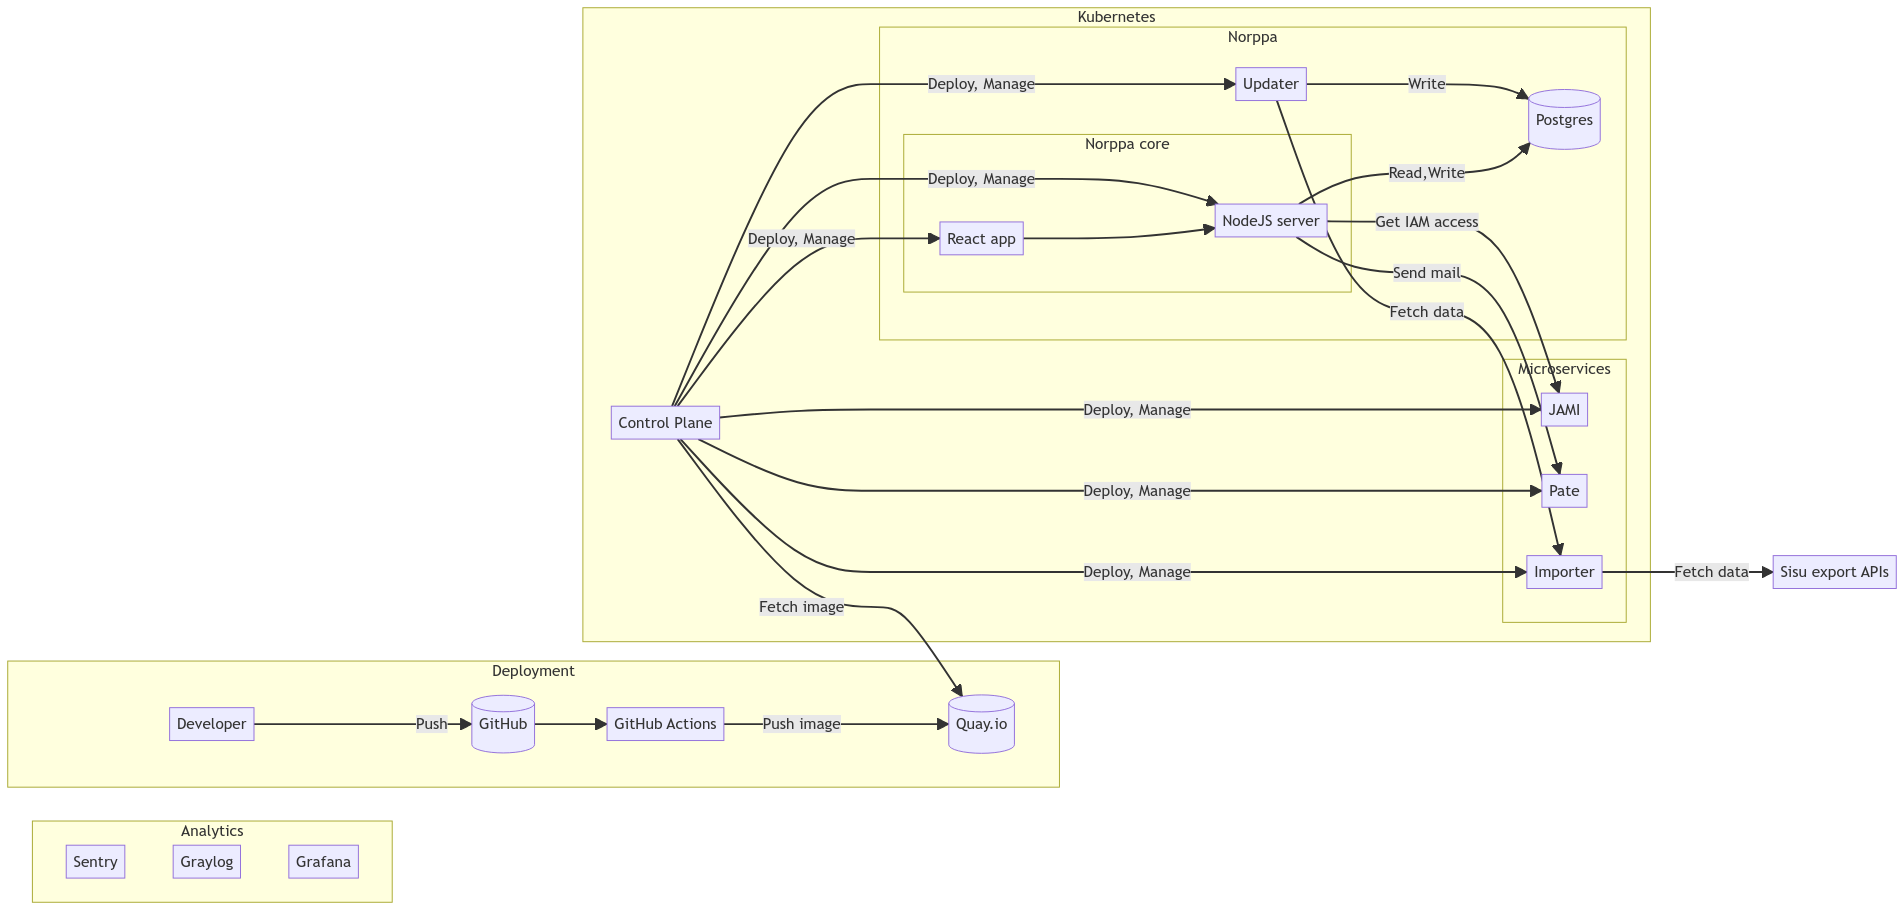
\includegraphics[width=1\textwidth]{figures/norppa_diagram.png}
\caption{Norppa-palautejärjestelmän laajennettu julkaisu- ja arkkitehtuuridiagrammi \cite{Norppa23}\label{fig:norppa}.}
\end{center}
\end{figure}
